\chapter{推理系统}
\label{chap:inference-systems}

\begin{keybox}[先弄清楚缓存了什么]
因果注意力保证旧 token 在某层的表示不会因后面追加新 token 而改变。生成下一个 token 时，该层只需要为新位置计算一行注意力：用新位置的 query 与所有可见位置的 key 匹配，再读取对应的 value。KV cache 保存每一层已经算过的历史 key 和 value，让旧位置不必随着每一步生成反复经过整层网络。
\end{keybox}

\section{从因果注意力到 KV cache}

设提示词已经有 \(x_1,\ldots,x_{t-1}\)，现在把新 token \(x_t\) 接在末尾。最直接的生成程序会把长度为 \(t\) 的整段前缀重新送入 Transformer，以取得位置 \(t\) 的输出，再预测 \(x_{t+1}\)。但这也重新计算了位置 \(1,\ldots,t-1\) 的 embedding、各层 Q/K/V、注意力和 FFN。因果 mask 使这些旧位置看不到新加入的 \(x_t\)，所以在模型参数不变时，旧位置在每一层的结果与上一步完全相同；重复计算它们没有必要。

看其中任意一层 \(\ell\) 的一个 attention head。令 \(u_i^{(\ell)}\) 是位置 \(i\) 送入该层注意力的向量；若该层采用 Pre-Norm，\(u_i^{(\ell)}\) 就是归一化后的层输入。投影得到 \(q_i^{(\ell)}=W_Q^{(\ell)}u_i^{(\ell)}\)、\(k_i^{(\ell)}=W_K^{(\ell)}u_i^{(\ell)}\) 和 \(v_i^{(\ell)}=W_V^{(\ell)}u_i^{(\ell)}\)。位置 \(t\) 的注意力输出为
\begin{equation}
 a_t^{(\ell)}=\operatorname{softmax}\!\left(
 \frac{q_t^{(\ell)}(K_{1:t}^{(\ell)})^{\mathsf T}}{\sqrt{d_k}}
 \right)V_{1:t}^{(\ell)},\qquad
 K_{1:t}^{(\ell)}=\begin{bmatrix}k_1^{(\ell)}\\ \vdots\\ k_t^{(\ell)}\end{bmatrix},\quad
 V_{1:t}^{(\ell)}=\begin{bmatrix}v_1^{(\ell)}\\ \vdots\\ v_t^{(\ell)}\end{bmatrix}.
 \label{eq:kv-cache-one-row}
\end{equation}
这一行只需要当前 token 的 \(q_t^{(\ell)}\)：先前 token 的 query 已用于计算各自的输出，现在不必重算。但是当前输出仍依赖从第 \(1\) 个到第 \(t\) 个 token 的所有 key 和 value，包括新 token 自己的 \(k_t^{(\ell)},v_t^{(\ell)}\)；key 决定匹配权重，value 提供被加权读取的内容。不同层的输入表示不同，因此每一层都要保存属于该层的先前 token 的 K/V，不能用某一层的缓存代替其他层。

实际生成时，模型保留各层旧位置的 \(K_{1:t-1}^{(\ell)},V_{1:t-1}^{(\ell)}\)。新 token 先得到当前层的输入向量，计算 \(q_t^{(\ell)},k_t^{(\ell)},v_t^{(\ell)}\)，把新 K/V 接到历史缓存后按式 \eqref{eq:kv-cache-one-row} 完成这一层的注意力，再经过输出投影、残差和 FFN，得到下一层所需的新位置表示；所有层依次完成后，词表头才预测下一个 token。缓存后续位置会反复读取的 K/V；对带 RoPE 的模型，缓存键还须带有相应的位置信息。

节省来自\textbf{旧位置不再重算}：每步只为新 token 做各层投影和 FFN，注意力也只算新位置这一行，从而省去整个前缀的 \(t\times t\) 个匹配分数重算。代价是每一步仍要读取长度为 \(t\) 的历史 K/V，所以注意力读取量随上下文线性增长，缓存显存也随生成长度增长。KV cache 不改变注意力公式或生成概率，只用存储历史中间结果换取较少的重复计算。

\section{Prefill 与 decode 是两个不同的计算问题}
\label{sec:prefill-decode}

用户给出一段长度为 \(P\) 的 prompt 时，首先要处理已经知道的这 \(P\) 个 token：一次送入整个 prompt，利用因果 mask 并行计算各位置在所有层的表示，同时填好各层位置 \(1,\ldots,P\) 的 KV cache。这一步叫 prefill；取最后一个位置的输出，经词表头得到 \(p_\theta(x_{P+1}\mid x_{1:P})\)，再采出第一个新 token。图 \ref{fig:prefill-decode} 把这一步与后续逐 token 生成并列画出。

采得 \(x_{P+1}\) 后，才进入逐步的 decode：把这个新 token 作为当前位置输入，用各层已有的 KV cache 计算它的表示，得到 \(p_\theta(x_{P+2}\mid x_{1:P+1})\)，同时把它自己的 K/V 写入缓存；后面的 token 重复同一过程。这里的 decode 指生成阶段，不要与 Transformer 架构中的 Decoder 层混为一谈。

两阶段使用同一模型，却有不同的计算形状。prefill 对整段 prompt 做大矩阵运算，一次计算并写入许多位置的 K/V，适合 GPU 的矩阵乘和融合注意力；decode 每步只有一个新 query，却要从显存读取全部历史 K/V，常受显存带宽和小矩阵效率限制。一个服务系统若只报告总 FLOPs，可能看不见 decode 的真实瓶颈。

这个差别也会进入硬件选择。prefill 更能利用高矩阵乘吞吐；decode 要长期容纳模型权重和不断增长的 KV cache，更看重显存容量与读取带宽，单纯增加算术吞吐未必同样有效。因而系统可以把两阶段放在不同的加速器或 GPU 资源池上，分别选择偏向计算或偏向存储的配置~\cite{patel2024splitwise}。这种分离引入 KV 传输：prefill 结束后必须把各层已建立的 KV cache 传给 decode 设备，若互连传输比节省的计算时间更贵，就可能得不偿失；第 \ref{sec:kv-budget} 节会估算这份状态的大小。

\begin{figure}[ht]
\centering
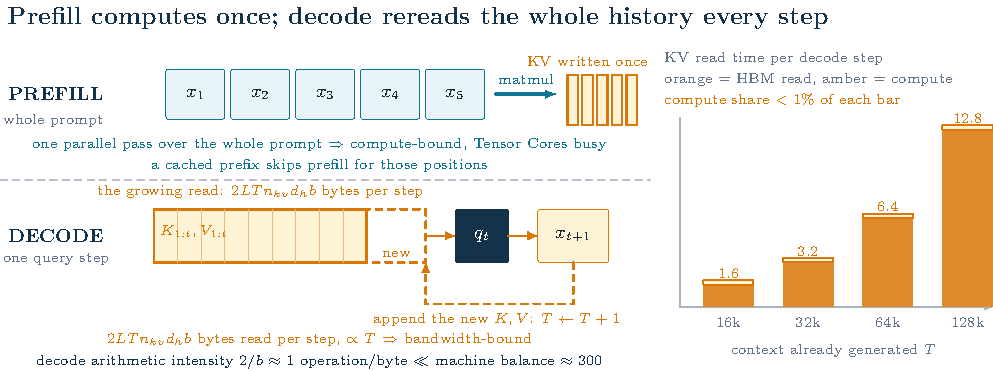
\includegraphics[width=\textwidth]{prefill_decode_cache.pdf}
\caption{prefill 对完整 prompt 并行计算并建立各层 KV cache；decode 每步计算一个新位置的 query、key 和 value，用新 query 读取历史 K/V，再把新 K/V 接到缓存中。}
\label{fig:prefill-decode}
\end{figure}

\section{KV cache 的数量级估算}
\label{sec:kv-budget}

对层数 \(L\)、KV heads \(n_{kv}\)、head dimension \(d_h\)、上下文 \(T\) 和元素字节数 \(b\)，标准 cache 近似为
\begin{equation}
 C_{\mathrm{KV}}\approx 2LTn_{kv}d_hb.
\end{equation}
这里的 2 来自 key 和 value 两份张量：每层、每个历史 token 各保存 \(n_{kv}d_h\) 个 key 元素和同样多的 value 元素，再乘层数、历史长度与每个元素的字节数。这个式子按单条请求计算，并假设 K/V 的 head 维度相同；多条并发请求的缓存容量还要按各自长度求和。
例如，假设 \(L=80\)、\(n_{kv}=8\)、\(d_h=128\)、\(T=128\,000\)、FP16 的 \(b=2\)，单请求全部 80 层的键和值总量约为
\begin{equation}
 2\times80\times128000\times8\times128\times2\ \text{bytes}\approx 39.1\ \text{GiB}.
\end{equation}
其中 \(1\,\mathrm{GiB}=2^{30}\) 字节。这是一个数量级估算，实际模型还会有层间布局、padding、量化、分组和并发请求；它足以说明为什么 GQA、MLA、paged cache 和长上下文调度很重要。

图 \ref{fig:attention-cache-variants} 在同一组 head 数和维度假设下比较 MHA、GQA、MQA 与 MLA 保存的历史状态。MHA 为每个 head 保存键和值；GQA 和 MQA 通过共享减少组数；MLA 保存低维表示和位置分支。具体比例取决于模型配置，所示百分比只对应标注的示例参数。

\begin{figure}[ht]
\centering
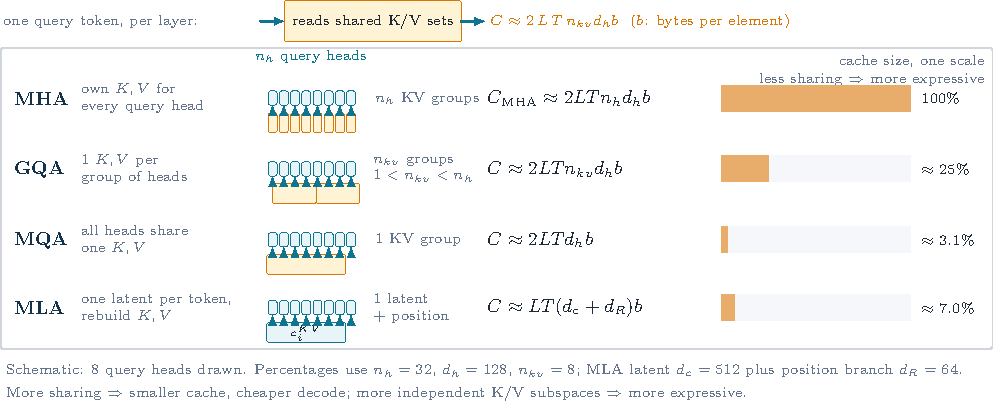
\includegraphics[width=\textwidth]{attention_cache_variants.pdf}
\caption{四种多头注意力形式的历史状态规模示例。图内给出用于计算百分比的 head 数、维度和潜变量大小；共享关系与表 \ref{tab:attention-variants} 一致。}
\label{fig:attention-cache-variants}
\end{figure}

\section{GPU 存储层级与输入输出（Input/Output，IO）感知注意力}

上一节的 KV cache 是生成期间长期保存的历史状态；这里的 FlashAttention 针对一次注意力计算中 \(T\times T\) 中间矩阵的临时读写。历史 K/V 的容量仍随上下文增长。

GPU 的高带宽显存（High Bandwidth Memory，HBM）容量大；更靠近计算单元的片上共享内存（shared memory）和寄存器（register）更快，但容量小。对长度为 \(T\) 的序列，普通注意力要计算每个 query 与每个 key 的匹配分数，形成 \(T\times T\) 的矩阵；每行做 softmax 后，再用得到的权重对 value 加权求和。如果把整张分数矩阵和权重矩阵写到 HBM、下一步再读回来，这些 IO 就会很耗时。

\Needspace{8\baselineskip}
FlashAttention 的 tiling 是把矩阵切成片上存储能容纳的小块~\cite{dao2022flashattention}。处理一小块 Q 时，依次读入各块 K 和 V，算当前块的匹配分数。每块先贡献给 softmax 分子中的 value 加权和、分母中的权重和；所有块处理完，才能得到最终输出。设 \(a_{ij}=q_i^{\mathsf T}k_j/\sqrt{d_k}\)，对本章的因果注意力，第 \(i\) 个 query 的输出为
\begin{equation}
 o_i=\frac{\sum_{j\le i}e^{a_{ij}}v_j}{\sum_{j\le i}e^{a_{ij}}}.
 \label{eq:flashattention-softmax-ratio}
\end{equation}
先暂时不考虑数值溢出。式 \eqref{eq:flashattention-softmax-ratio} 的分子、分母都是求和。把可见的 key 位置分成若干块，给每个 query 行分别设累计分母 \(Z_i=0\) 和累计分子 \(U_i=0\)；读入一个 K/V 块 \(B\)，只需更新
\begin{equation}
 Z_i\leftarrow Z_i+\sum_{j\in B}e^{a_{ij}},\qquad
 U_i\leftarrow U_i+\sum_{j\in B}e^{a_{ij}}v_j,\qquad
 o_i=\frac{U_i}{Z_i}\quad\text{（全部块结束后）}.
 \label{eq:flashattention-online-softmax}
\end{equation}
例如第一块只有 \(a=0,v=10\)，更新后 \(Z_i=1,U_i=10\)；第二块只有 \(a=\ln 2,v=20\)，因为 \(e^{\ln 2}=2\)，它给分母增加 \(2\)、给分子增加 \(40\)，于是 \(Z_i=3,U_i=50\)，最终输出为 \(50/3\)。一次性对两项做 softmax，权重比也是 \(1:2\)，结果相同。“在线”就是每来一块便更新这两个累计量；各块提供的是部分和，归一化留到最后。

实际计算还要避免 \(e^{a_{ij}}\) 过大而溢出。于是每个 query 行另存一个已处理分数的最大值 \(m\)，把指数改写成 \(e^{a_{ij}-m}\)，并以这个基准保存分子和分母。若新块把最大值提高到 \(m'\)，旧的两个累计量都先乘 \(e^{m-m'}\)，再加入按 \(m'\) 计算的新块；这样新旧贡献始终使用同一基准。图 \ref{fig:gpu-memory} 展示了这个读写顺序。FlashAttention 保留逐对 Q--K 匹配，省去的是完整 \(T\times T\) 中间矩阵在 HBM 中的写入与读回。后续 FlashAttention-2 改进并行与工作划分~\cite{dao2023flashattention2}；FlashAttention-3 进一步利用异步执行和低精度计算~\cite{dao2024flashattention3}。

\begin{figure}[ht]
\centering
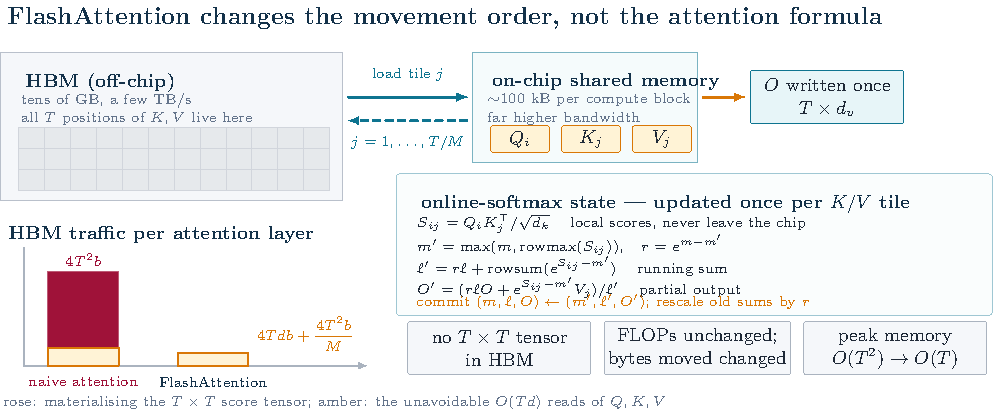
\includegraphics[width=\textwidth]{flashattention_io.pdf}
\caption{FlashAttention 改变矩阵分块与搬运顺序：从 HBM 读入一块 Q 和各块 K/V，在片上累加 softmax 分子与分母，处理完所有 K/V 块后才得到最终输出，避免物化完整的 $T\times T$ 中间矩阵。}
\label{fig:gpu-memory}
\end{figure}

\section{分页缓存、结构化服务与推测解码}
\label{sec:paged-serving}

当多个请求同时生成时，每条历史的长度不断变化，预先分配连续大块显存容易浪费空间。推理引擎 vLLM 的 PagedAttention 借鉴虚拟内存，把 KV cache 切成固定大小的 block，让不同请求的前缀共享物理页面并减少碎片~\cite{kwon2023vllm,vllmblog}。结构化生成语言与运行时 SGLang（Structured Generation Language）进一步把多次生成与工具调用组织成程序。其 RadixAttention 用前缀树索引可复用的历史缓存；连续批处理则在每轮生成后及时加入新请求、移除已完成请求，适合多轮对话、工具调用、树状推理和多个分支共享前缀的场景~\cite{zheng2024sglang,sglangdocs}。智能体每一轮都把上一轮的完整输入作为前缀重新提交，是这种前缀复用最典型的负载，见第 \ref{chap:agents} 章。

例如请求 A 正在逐 token 生成时，请求 B 完成 prefill 并取得首 token。连续批处理可以在下一轮 decode 把 B 加入正在运行的 batch，A 完成后则把它移出；B 不必等 A 生成完整段文字。两条请求的历史长度不同，分页缓存分别记录它们的 KV 页面，调度器在每轮为各请求安排一个新位置。

分页之后紧接着是缓存容量管理。对\textbf{可复用前缀缓存}，显存不足时可按最近使用时间或请求优先级回收页面；以后若再次需要这段前缀，缓存未命中就重新做 prefill，计算结果仍与未淘汰时一致。另一类方法会按注意力分数等指标丢弃活跃请求中较少被读取的历史 K/V，以减少后续读取；此时当前 token 可见的历史已改变，注意力结果只是近似。两类方法节省的显存相似，计算代价和对输出的影响却不同。

另一项调度选择是\textbf{prefill 与 decode 分离（Prefill-Decode Disaggregation，PD 分离）}。第 \ref{sec:prefill-decode} 节说明了这两个阶段的计算特征相反：prefill 是大矩阵乘、计算受限，decode 是逐 token、带宽受限。把它们放在同一批 GPU 上调度，两边的效率都会受损——一个长 prompt 的 prefill 会阻塞正在 decode 的请求，造成明显的首 token 与 token 间延迟抖动。PD 分离把两类工作放到不同的 worker 池：prefill 池负责处理输入并生成 KV，再通过高速网络把 KV 传给 decode 池，decode 池只做逐 token 解码。

这个方案把“计算组织”的权衡摆到了读者面前。收益是两类阶段都可以按各自最优的并行策略和 batch 形状运行，且各自独立扩缩容；代价是 KV cache 需要跨节点传输，传输量恰好等于第 \ref{sec:kv-budget} 节估算的那个体积，因此 PD 分离是否划算取决于网络带宽与 KV 大小之比。对长上下文和长输出场景，这个比值通常是有利的；对短请求，传输开销可能吃掉全部收益。DeepSeek-V4 与 Kimi K3 把“异构 cache 的 offload/prefetch”和“外部 KV pool”写进系统设计，处理的正是这一步带来的数据搬运问题。

要看清 PD 分离改善了什么，需要分开记录服务指标。按本章的生成顺序，请求先等待并完成 prefill，由末位置输出首 token；随后传输 KV，decode 池才用这个 token 继续生成。首 token 时间（Time to First Token，TTFT）从请求到达到首 token 返回；相邻 token 间延迟（Inter-Token Latency，ITL）记录连续两次输出之间的等待；吞吐量则统计单位时间内所有请求共同完成的 token 数。

\begin{table}[ht]
\centering\small
\begin{tabularx}{\textwidth}{>{\raggedright\arraybackslash\bfseries}p{34mm} X X}
\toprule
指标 & 主要由什么决定 & PD 分离可能带来的变化\\
\midrule
首 token 时间 TTFT & prefill 排队、prompt 计算与首 token 返回 & 专用 prefill 池可减少与 decode 的资源争用；若实现要等 KV 传完才返回首 token，传输也进入这一指标\\
后续 token 间延迟 ITL & decode 排队、每轮计算与历史 KV 读取 & decode 不再被长 prefill 打断；但首 token 到第二个 token 的间隔还可能包括 KV 传输与 decode 池入队\\
总吞吐量 & 两个池各自的处理能力及请求混合 & 两阶段可分别配 batch 和扩容；若 KV 传输或任一池排队成为瓶颈，吞吐未必提高\\
\bottomrule
\end{tabularx}
\caption{PD 分离对服务指标的影响。表述按首 token 由 prefill 阶段产生的流程；具体返回时机和网络传输是否重叠取决于实现。}
\label{tab:pd-serving-metrics}
\end{table}

speculative decoding 使用较小的 draft model 生成候选 token，大模型批量验证~\cite{leviathan2023speculative}。如果接受规则设计正确，最终输出保持目标模型的分布；系统收益来自把串行目标模型调用变成“少量 draft 串行 + 一次目标模型并行验证”。这次验证仍计算多个候选位置，主要节省的是目标模型逐 token 调用的串行等待。这是工程加速通过改变计算组织而保持目标概率分布不变的一个典型例子。

\begin{figure}[H]
\centering
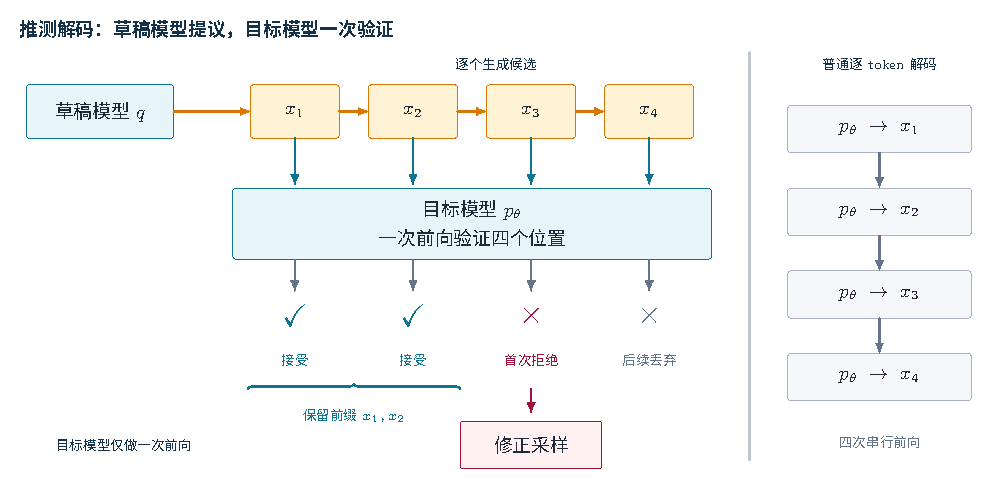
\includegraphics[width=\textwidth]{speculative_decoding.pdf}
\caption{推测解码：小模型串行提出四个候选，目标模型一次计算各候选位置的条件概率，再从左到右判定是否接受。图中前两个候选被接受，第三个被拒绝并修正采样，第四个随之丢弃；正确接受规则保持目标模型的输出分布。}
\label{fig:serving-stack}
\end{figure}
